\documentclass[12pt, a4paper]{article}

\usepackage[utf8]{inputenc}
\usepackage[francais]{babel}
\usepackage{meeting}
\usepackage{xcolor}
\setcounter{section}{-1}
\title{Mode d'emploi du projet}


\author{Schwing, Roug\'e, Moulin, Chaput, Toulisse}

\date{\today}

\begin{document}

\maketitle

\section{"Mode d'emploi"}

Les programmes sont compilés à l'aide de la commande "make".
Tous les programmes utilitaires sont lancés dans projet.c.
		
La commande ./projet permet d'exécuter le programme et comporte plusieurs options d'affichage.

L'option -f est indispensable, doit être suivie du fichier étudié et mise directement après ./projet.	
"./projet -f "nom_du_fichier"

Les autres options sont mises après le nom du fichier et sont :
		- h : affiche l'en-tête du fichier
		- S : affiche les en-têtes de section
		- s : affiche la table des symboles
		- r : affiche les informations des tables de relocalisation
		- H : affiche une aide pour l'utilisation de la commande ./projet
		- x "numéro ou nom section": Cette option doit être mise en dernière avec le numéro ou nom d'une section à la suite.
					Elle permet d'afficher le contenu de la section donnée en paramètre.

En sortie deux fichiers test*.o sont crées dans le répertoire courant, un sans les tables de réallocations et un avec toutes les réadressages des sections.

Enfin le nettoyage des fichier.o se fait avec la commande "make clean".

\section{"Structure de fichiers"}
\begin{figure}[!h]
    \begin{center}
        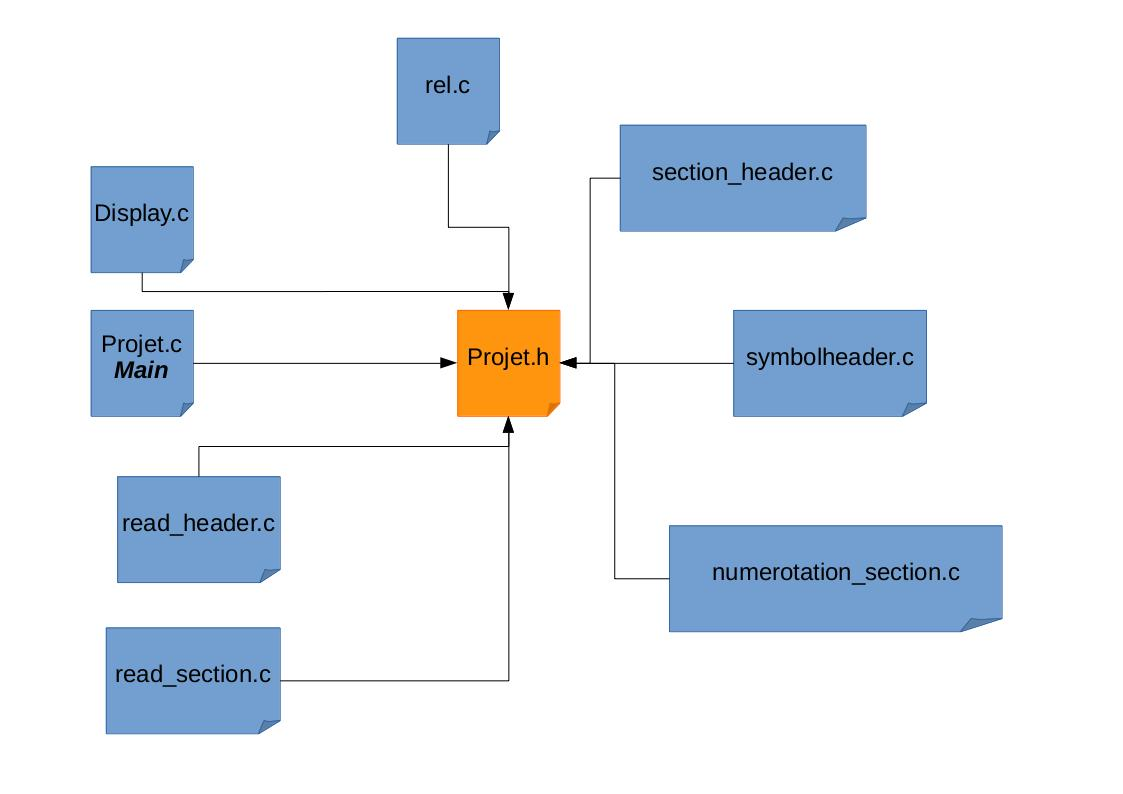
\includegraphics[width=\textwidth]{archi_projet.jpg}
        \caption{Nagvis backend configuration}
    \end{center}
\end{figure}

Le projet s'articule autour de 8 fichiers : 

un fichier projet.h contenant la déclaration de toutes les fonctions et structures du projet

un fichier read_header.c contenant les fonctions nécessaires à la lecture du header d'un fichier ELF (partie 1)

un fichier section_header.c contenant les fonctions nécessaires à la lecture de la table des sections (partie 2)

un fichier read_section.c contenant les fonctions nécessaires à la lecture du contenu des sections (partie 3)

un fichier symbolheader.c contenant les fonctions nécessaires à la lecture des symboles du fichier ELF (partie 4)

un fichier rel.c contenant les fonctions nécessaires à la lecture des sections de réimplémentation (partie 5)

un fichier display.c permettant d'afficher le résultat de chacune des tâches précédentes

un fichier projet.c contenant la fonction principale du projet.
\end{document}

